\documentclass{article}
\usepackage[utf8]{inputenc}

\title{Lecture 8: Linear Algebra  }
\author{wbg231 }
\date{November 2022}
\usepackage{tikz,graphicx,amsmath,amsfonts,amscd,amssymb,bm,cite,epsfig,epsf,url}
\begin{document}

\maketitle

\section{Linear algebra introduction}
\subsection{vectors}
\begin{itemize}
%\item 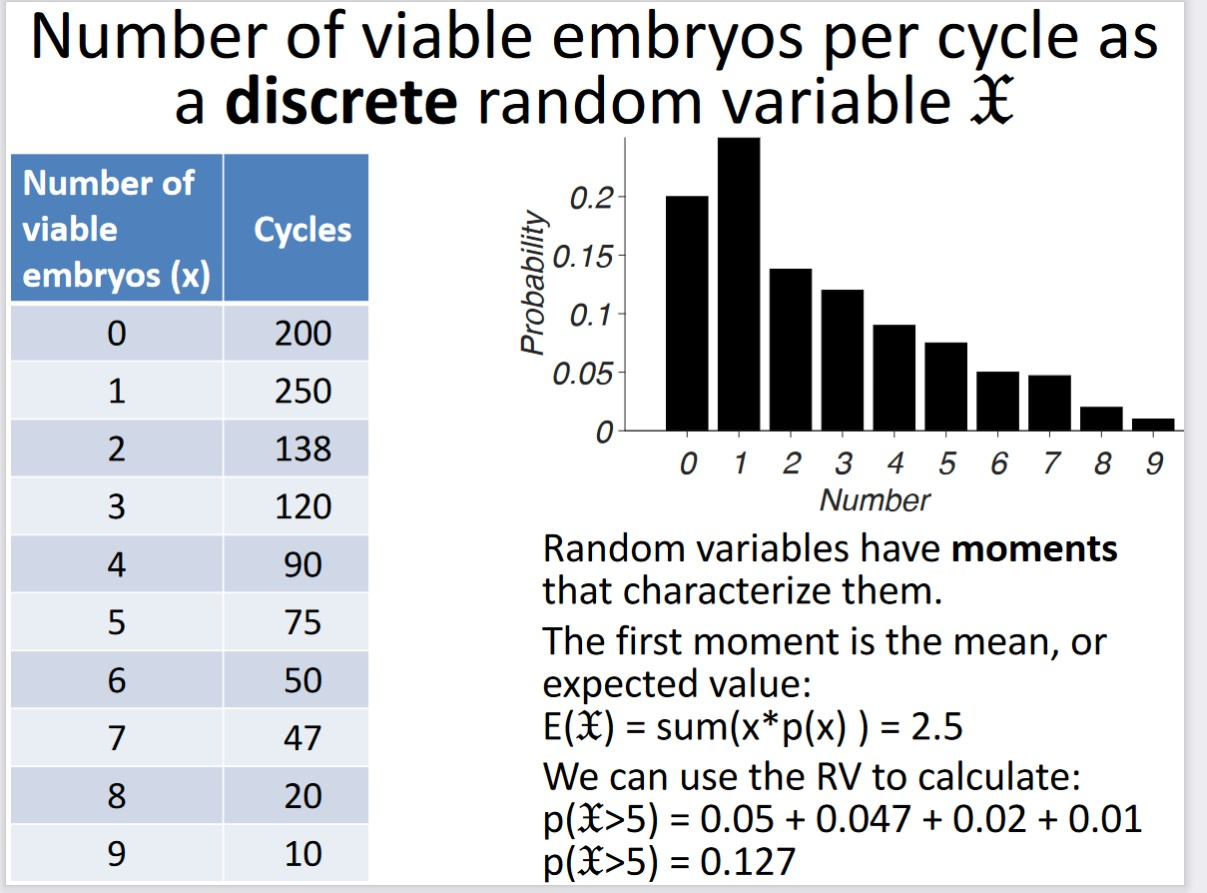
\includegraphics[width=7.5cm]{Final_Review/Lecture_2/lecture_1example.jpg}
\item real numbers can be represented as locations on the real number line 
\item vectors are stacks of numbers linear algebra is the study of vectors and the operations on them 
\item v=\begin{pmatrix}
1\\2\end{pmatrix}
\item vectors have different location deepening on the field 
\item in cs they are really just lists of Numbers 
\subsection{vector operation}
\item for a set to be a vector space, it must have scalar multiplication and vector addition well deafened. 
\item scalar multiplication changes the length but not the direction, they scale the vector
\item vector addition just is element wise. and you can draw there sum as an arrow form the origin to the coordinates of the sum
\item if these things hold then something is a vector 
\item in math a vector can be a set of anything 
\item in cs a vector can be a list of numbers 
\item in DF we are only dealing with data with a finite dimension 
\item vector is usually written as lower case bold \mathbf{v} is a vector i am just going to write it as normal lower case numbers 
\item unless otherwise specified the default vector is a column vector ie $v\in \mathbb{R}^n=v\in \mathbb{R}^{1XN}$
\item so the transpose of a vector just is a row vector usually 
\item we use vectors to represent data. this is often a way to speed up computation
\subsection{why are vectors use full}
\item all currencies can be expressed in terms of each other so a scalar is enough to have account for money 
\item but if we have money and height that we want to represent a vector is a good idea as we can compare the heights and the money
\subsection{dot product}
\item $x,y\in \mathbb{R}^N$ the dot product is $x*y=<x,y>=x^ty=\sum_{i=1}^{n}x_iy_i=\alpha\in\mathbb{R}$ 
\item there are other products, but we are mainly focused on the dot product.
\subsection{Geometric interpretations of the dot product}
\item linear algebra is nice because it is geometrically inheritable 
\item $x*y=||x||*||y||*cos(\theta)$ where theta is the angle between them this can be expressed as $cos(\theta)=\frac{<x,y>}{||x,x||*||y||}$
\item this allows us to tell how similar vectors are 
\item the dot product between vectors help us understand similarity. this leads to correlation
\subsection{vector projection}
\item suppose we have a data point b that we want to project onto a subspace
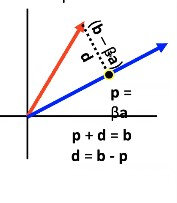
\includegraphics[width=7.5cm]{Final_Review/lecture_8/vector_projection.jpg}
\item in the standard position coordinates are directions \item so we are looking for a $\beta\in \mathbb{R}$ such that $\beta a$ is as close to b with out leaving a as possible 
\item a is predictor b is outcome. 
\item let $\beta a$ be a projected onto b. 
\item we know that the distance from b to $\ba$ is $d=b-\beta a$ and that d must be orthogonal to a. (this is more or less because we are taking away the movement of b in the direction of a 
\item so in other words we know that $0=<d,\beta a>=<b-\beta a, \beta a>=<b,\beta a>-<\beta a, \beta a>=\beta<a,b>-\beta^2<a,a>=0$ meaning that $\beta<a,b>=\beta^2<a,a>\Rightarrow \beta =\frac{<a,b>}{<a,a>}$ so this is the regression $\beta$
\item in other words linear regression can just be written as a dot product
\tem think of the vector projection as the shadow a vector casts on a space
\subsection{outer product}
\item the outer product of two vectors x and y is the matrix of the transpose of the matrix product of the first times the second  $v\otimes x=v^tx\in \mathbb{R}^{n,n}$
\item this outputs a matrix
\item form this perspective we can think of a matrix as a stack of vectors
\subsection{matrices}
\item matrix are stack of vectors 
\item a matrix can give many determinants. 
\item matrix are written as single upper case Numbers 
\item the determinate of a matrix is only def fined for square matrix, it is basically how the area of the basis vectors are changed by the linear transformation matrix.
\item if det(A)=0 then rank(a) is less than n 
\subsection{matrix multiplication}
\item Ax=b $A\in \mathbb{R}^{nXm}, x\in \mathbb{R}^{m} b\in \mathbb{R}^{n}$
\item a matrix is a linear transform that can act on a vector
\item matrix multiplication is a just dot products
\item the transpose of a matrix is flipping it \subsection{matrix in data science}
\item we represent multivariate data sets as matrix in data science
\subsection{eigenvectors and values}
\item usually $Ax$ will rotate and stretch x.
\item an eigenvector is a vector such that $Av=\lambda v$ ie multiplying v by a just stretches it by some scalar. 
\subsection{ dimensionality  reduction}
\item a line through the pole of the earth would be its eigenvector because as the earth rotates that line does not move
\subsection{example}
\item modeling predator prey dynamics 
\item foxes eat hairs, hairs reproduce
\item  we can represent this as a matrix and find the eigen vectors
\item these eigenvalues tell us the long term behavior of the system 
\item the eigenvectors are the point of stable growth effectively 
\subsection{where do eigen vectors come from}
    \item matrix factorization, ie we can compose a matrix in to upper and lower triangle matrices to solve systems of linear equations 
\subsection{factoring matrices}
\item factoring numbers is useful because it simplifies things and component parts can be useful
\item in our class the two factoring methods that matter are the eigen decomposition which factors square symmetric mercies into orthogonal eigen vectors and values 
\subsection{SVD}
\item alows us to decompose any matrix uniquly into 3 componets each of with is interpreatble $A=u\Simga V^T$
\item U,V are orthogonal. that means they are square, the rows and cols are orthogonal, it is really just a rotation. invariant to length and angles, and the inverse is the transpose
\item diagonal matrix just stretches space, it can be easily inverted
\item SVD yields a unique decomposition that is composed of rotation and stretching components. 
\item this matters because this allows us to easily work with parts of the matrix
\item these are used everywhere 
\item 
\end{itemize}

\end{document}
